\section{Deep Convolutional Neural Network: U-Net}
\label{sec:Model}
Zur Verarbeitung von Bildern haben sich in der Vergangenheit Convolutional Neural Networks (CNNs) bewiesen.
Grundsätzlich besteht ein CNN aus mehreren Convolutional Ebenen, gefolgt von einer Pooling Ebene.
Wird von einem tiefen CNN gesprochen, so ist damit ein Netzwerk aus mehreren CNN-Einheiten gemeint.
\\
Die hier verwendete CNN-Struktur wird als U-Net bezeichnet und gehört zu den tiefen CNNs.
Das U-Net gewann $2015$ zwei Challanges, zum einen für automatische Computerdetektion von Karies in Bissflügel-Röntgenaufnahmen (ISBI $2015$) und zum anderen die Erkennung von Zellen (ISBI $2015$).\cite{RFB15a}
Bis heute sind Modelle dieser Art eine beliebte Wahl bei Segmentierungen.

\subsection{Architektur}
Die verwendete Netzwerkstruktur ist in \autoref{tab:structure} aufgeführt und in \autoref{fig:unet_structure} visuell dargestellt.
Das U-Net besteht dabei aus einem absteigenden und einem aufsteigenden Ast, ähnlich wie bei einem Auto-Encoder.
Zusätzlich sind Lagen aus dem Encoder direkt mit Lagen aus dem Decoder verknüpft (siehe Pfeile in gen. Abb.).
Die Daten werden hier lediglich kopiert und über die Verkettungs-Lage mit den vorherigen Daten zusammengefügt.
\\
Ein wie in der genannten Abbildung dargestellter Block (oder CNN-Einheit) im aufsteigendem Ast besteht aus einer Convolutional Lage, gefolgt von einem Dropout, einer weiteren Convolutional Lage und einer Max Pooling Schicht.
In der Convolutional Lage wird, wie der Name schon sagt die diskrete Faltung berechnet.
Mithilfe dieser Lage können bei der Bildverarbeitung Bereiche indentifiziert werden.
Durch die Einstellung 'padding = same' ist sichergestellt, dass die Bildgröße unverändert bleibt.
\\
Die Max Pooling Ebene bewegt sich dabei über die Eingabe und speichert den maximalen Wert.
Dabei werden überflüssige Informationen verworfen und die Dimension des Bildes verkleinert.
\\
Im absteigenden Ast besteht eine CNN-Einheit aus einer Convolutional Lage, gefolgt von einem Dropout, einer weiter Convolutional Lage, einer Transposed Convolutional Lage und endet mit einer Verkettungsebene.
Hier wird die Bildgröße wieder erhöht, daher wird statt der MaxPooling eine Transposed Convolutional Lage verwendet.
\\
Um das Übertrainieren des Netzes zu verhindern, wird in jedem CNN-Block ein Dropout verwendet.
Der Dropout steigt um $0.1$ alle zwei CNN-Einheiten für den aufsteigenden Ast (mit der Tiefe des Netzes).
Der maximale Dropout wird bei der mittleren CNN-Einheit erreicht.
Bei dem aufsteigendem Ast wird der Dropout wieder um $0.1$ je zwei CNN-Einheiten reduziert.
\\
Analog dazu wird die Filtergröße der Convolutional Lage mit der tiefe pro CNN-Einheit verdoppelt bzw. beim aufsteigenden Teil halbiert.
Die Filtergrößen der einzelnen Convolutional Lagen sind zur Verdeutlichung in \autoref{fig:unet_structure} eingezeichnet.
In der letzten Lage wird die Sigmoid-Funktion und in den restlichen Convolutional Lagen die Rectifier Aktivierungsfunktion (ReLU) verwendet.
\\
Zudem wird Adam als Optimierer festgelegt.
Als Verlustfunktion wird die binäre Kreuzentropie eingesetzt, da diese eine gute Wahl für Klassifizierungsprobleme mit zwei Klassen ($0$/Land oder $1$/Wasser) ist.
Das Modell wird über die Genauigkeit bewertet, d.h. der Anteil der übereinstimmenden Pixel der vorhergesagten Bilder mit der Maske.
\\
Die Wahl der Hyperparameter wird im folgenden \autoref{sec:Hyperparameter} erläutert.
\begin{figure}
    \centering
    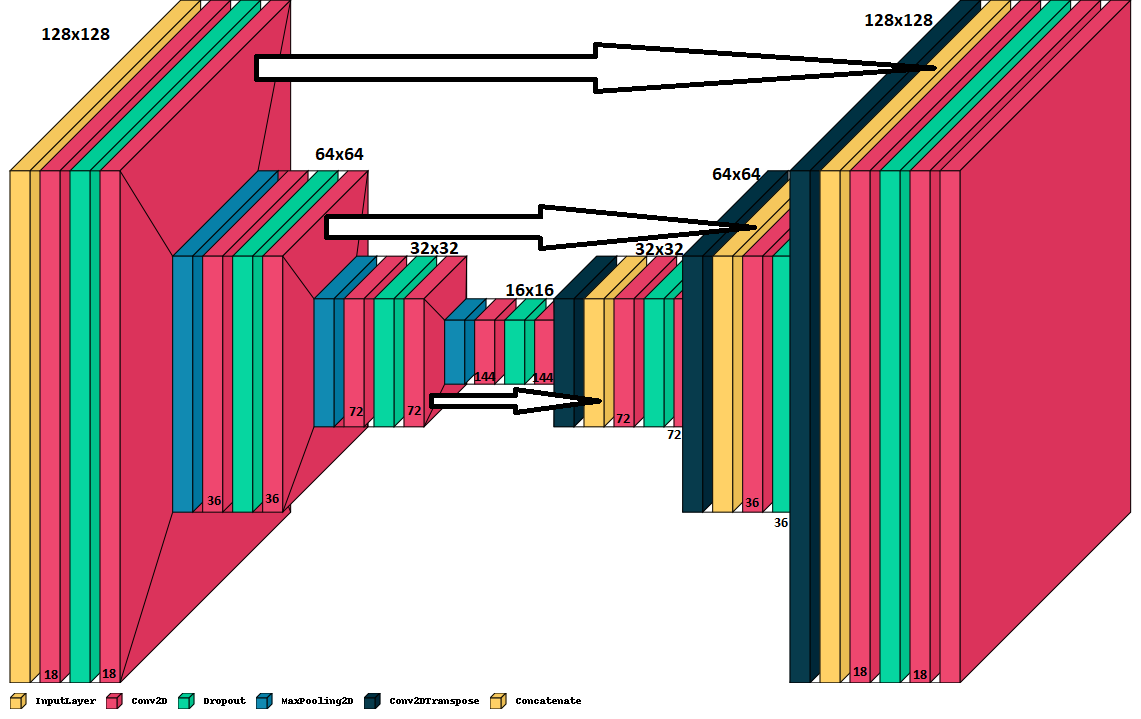
\includegraphics[width=0.8\textwidth]{content/img/unet_struc_bearbeitet_2.png}
    \caption{Schematische Darstellung der verwendeten Netzwerkstruktur: U-net. (VisualKeras)}
    \label{fig:unet_structure}
\end{figure}

\FloatBarrier

\subsection{Optimierung der Hyperparameter}
\label{sec:Hyperparameter}
Zur Bestimmung der optimalen Hyperparameter wurde eine zufällige Gittersuche durchgeführt.
D.h. es werden nach dem Zufallsprinzip Parameter gewählt und mit diesen das Modell trainiert und evaluiert.
Auf eine vollständige Gittersuche wurde aufgrund der hohen Rechenzeit verzichtet.
\\
Es wurden $3000$ Daten zum Trainieren und $3000$ zum Validieren verwendet.
Insgesamt wurden $100$ Modelle mit einer Batchsize von $128$ und Epochenanzahl von $20$ trainiert und ausgewertet.
Die Ergebnisse der einzelnen Parameter sind in \autoref{fig:grid_ergebnisse} graphisch dargestellt.
\begin{figure}
    \centering
    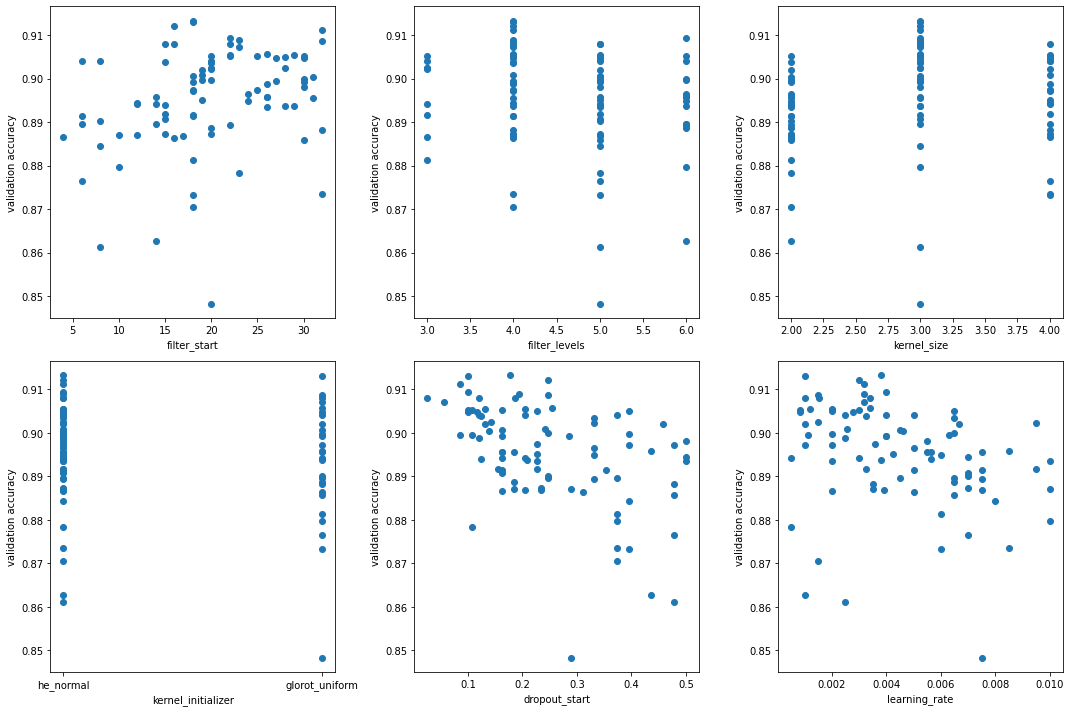
\includegraphics[width=0.95\textwidth]{content/img/grid_ergebnisse.png}
    \caption{Die Genauigkeit zu den sechs variierten Parametern der zufälligen Gittersuche.}
    \label{fig:grid_ergebnisse}
\end{figure}
\FloatBarrier
Die Wahl des 'Kernel Initialisierer' scheint kaum Einfluss auf die Genauigkeit zu haben.
Hingegen ist bei der Lernrate und beim Startwert der Dropoutrate bzw. der Filteranzahl ein Trend zu erkennen.
Eine geringe Dropout- und Lernrate bzw. eine größere Filteranzahl deutet auf eine höhere Genauigkeit hin.
Ebenso sollte eine $3\times3$ Kernelgröße der Convolutional Ebene und eine U-Net Tiefe von $4$ gewählt werden.

Das Modell mit der höchsten Genauigkeit auf den Validierungsdaten, wurde anschließend auf allen Daten ($\thicksim \SI{58000}{}$) trainiert.
\begin{table}
    \centering
    \caption{Die fünf besten Modelle, absteigend nach der höchsten Genauigkeit auf den Validierungsdaten sortiert.}
    \label{tab:grid_best}
    \begin{tabular}{S[table-format=2.0] S[table-format=1.0] S[table-format=1.0] l S[table-format=1.6] S[table-format=1.6] | S[table-format=1.6]}
        \toprule
        {Filter} & {Tiefe} & {Kernelgröße} & {Kernel Init.} & {Dropout} & {Lernrate} & {Val. Genauigkeit} \\
        \midrule
        18 & 4 & 3 & He Normal & 0.177895 & 0.003795 & 0.913355 \\
        18 & 4 & 3 & Glorot Uniform & 0.100000 & 0.001000 & 0.913100 \\
        16 & 4 & 3 & He Normal & 0.247368 & 0.003000 & 0.912037 \\
        32 & 4 & 3 & He Normal & 0.086316 & 0.003179 & 0.911288 \\
        22 & 6 & 3 & He Normal & 0.100000 & 0.004000 & 0.909450 \\
        \bottomrule
    \end{tabular}
\end{table}
\FloatBarrier

\subsection{Training und Schwellenwert}
Das Modell, welches die besten Ergebnisse ($\text{Validierungs Genauigkeit} = \SI{91.34}{\percent}$) in der Gittersuche erzielte (siehe erster Eintrag in \autoref{tab:grid_best}), wurde dann auf dem ganzen Datensatz trainiert und evaluiert.
Es hat sich gezeigt, dass eine hohe Batchgröße eine postive Auswirkung auf die Genauigkeit hat.
Aufgrund des limitierten Arbeitsspeichers wurde die maximal mögliche Batchgröße von $128$ gewählt und das Modell über $50$ Epochen trainiert.
Aus der Epoche mit der höchsten Validierungs Genauigkeit wird das Modell gespeichert.
Der Verlauf der \textbf{Genauigkeit} und der \textbf{Verlustfunktion} des Modells auf dem gesamten Datensatz, kann in \autoref{fig:loss_acc} betrachtet werden.
\begin{figure}
    \centering
    \begin{subfigure}{0.48\textwidth}
        \centering
        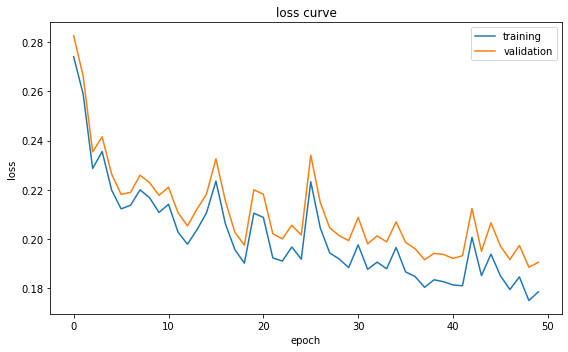
\includegraphics[width=\textwidth]{content/img/loss.png}
        \caption{Verlustfunktion}
    \end{subfigure}
    \begin{subfigure}{0.48\textwidth}
        \centering
        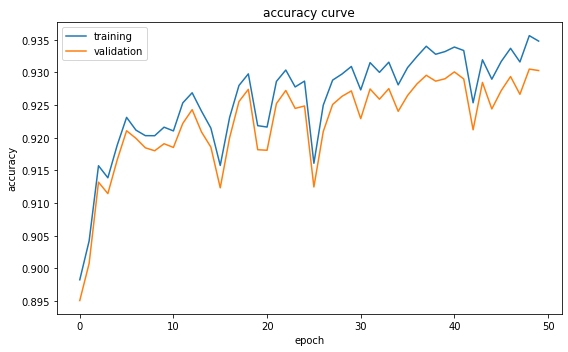
\includegraphics[width=\textwidth]{content/img/acc.png}
        \caption{Genauigkeit}
    \end{subfigure}
    \caption{Verlauf der Genauigkeit und der Verlustfunktion über die Epochen.}
    \label{fig:loss_acc}
\end{figure}

Der Verlust und die Genauigkeit für Validierungs- und Trainingsdaten unterscheiden sich minimal.
Es gibt keine Anzeichen für ein übertrainiertes Modell.
Grund dafür ist zum einen der verwendete Dropout, aber auch die Größe des Datensatzes.
Das Neuronale Netz mit $\sim \SI{600000}{}$ trainierbaren Parameter hat nicht die Möglichkeit sich an der großen Anzahl an Daten anzupassen bzw. die Bilder auswendig zu lernen.
\\
Aufgrund der in der finalen Ebene verwendeten Aktivierungsfunktion 'Sigmoid', werden als Ausgabe Pixelwerte zwischen $0$ und $1$ generiert.
In \autoref{fig:count_values} ist die Verteilung der Pixelwerte für Wasser bzw. kein Wasser dargestellt.
\\
Es handelt sich weiterhin um ein binäres Klassifizierungsproblem, daher wird ein \textbf{Schwellenwert} gesetzt.
Liegt der Wert eines Pixels über bzw. unter dem Schwellenwert, so wird dieser als Wasser bzw. kein Wasser klassifiziert.

Um den optimalen Schwellenwert zu finden, wird die Genauigkeit auf den Validierungsdaten in Abhängigkeit des Schwellenwerts betrachtet. (siehe \autoref{fig:schwellenwert})

\begin{figure}[ht]
    \centering
    \begin{minipage}[t]{0.464\linewidth}
        \centering
        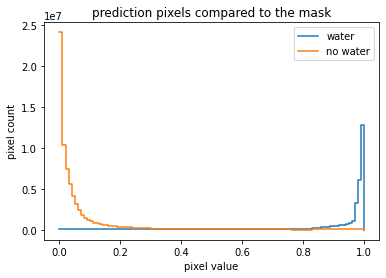
\includegraphics[width=\textwidth]{content/img/pixel_values_counter.png}
        \caption{ }{\small{Darstellung der Häufigkeit der vorhergesagten Pixelwerte.}}
        \label{fig:count_values}
    \end{minipage}%
    \begin{minipage}[t]{0.48\linewidth}
        \centering
        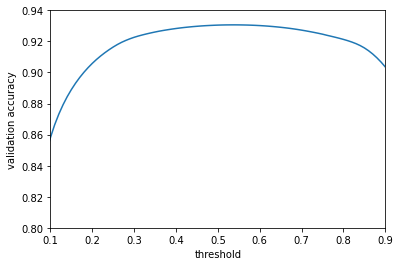
\includegraphics[width=\textwidth]{content/img/schwellenwert.png}
        \caption{ }{\small{Validierungs Genauigkeit in Abhängigkeit des Schwellenwerts.}}
        \label{fig:schwellenwert}
    \end{minipage}
\end{figure}

Die maximale Validierungs Genauigkeit $\SI{93.07}{\percent}$ wird beim Schwellenwert $S = \SI{0.54}{}$ erreicht.

\begin{figure}
    \centering
    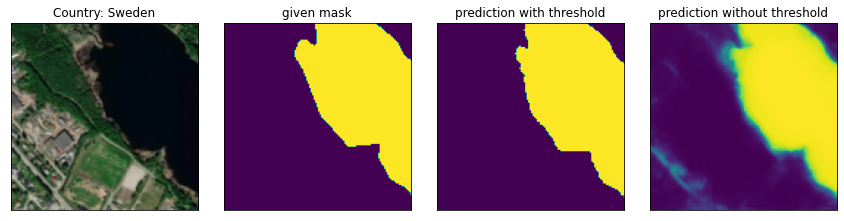
\includegraphics[width=0.9\textwidth]{content/img/threshold_img.png}
    \caption{Typ der Bilder von links nach rechts: Satellitenbild, Maske, Vorhersage mit Schwellenwert, unbearbeitete Vorhersage. \copyright Mapbox, \copyright OpenStreetMap}
    \label{fig:threshold_img}
\end{figure}
\autoref{fig:threshold_img} stellt die Aufgabe des Schwellenwerts anhand eines Beispiels dar.
Der Pixelwert ist ein Maß für die Wahrscheinlichkeit, ob sich an dieser Stelle Wasser befindet.
Wie in dem Beispielbild zu sehen, wird der blaue Bereich links unten nach setzten des Schwellenwerts nicht mehr als Wasser eingestuft, was auch mit der Maske übereinstimmt.
Weitere Ergebnisse können in \autoref{sec:vergleich}: \enquote{CNN und Random Forest im Vergleich} betrachtet werden.